%++++++++++++++++++++++++++++++++++++++++++++++++++++++++++++++++++++++++++++++
% Para alterar o TIPO DE DOCUMENTO, preencher a linha abaixo \documentclass[?]{?}
%   \documentclass[tg]{ita}			= Trabalho de Graduacao
%   \documentclass[tgfem]{ita}	= Para Engenheiras
%   								msc     		= Dissertacao de Mestrado
%   								mscfem   		= Para Mestras
%   								dsc      		= Tese de Doutorado
%   								dscfem   		= Para Doutoras
%   								quali    		= Exame de Qualificacao
%   								qualifem 		= Exame de Qualificacao para Doutoras
% Para 'Draft Version'/'Versao Preliminar' com data no rodape, adicionar 'dv':
%   \documentclass[dsc, dv]{ita}
% Para trabalhos em Inglês, adicionar 'eng':
%   \documentclass[dsc, eng]{ita}
%		\documentclass[dsc, eng, dv]{ita}
%++++++++++++++++++++++++++++++++++++++++++++++++++++++++++++++++++++++++++++++
\documentclass[mscfem,dv, eng]{ita}    % ITA.cls based on standard book.cls
% Quando alterar a classe, por exemplo de [msc] para [msc, eng]) rode mais uma vez o botão BUILD OUTPUT caso haja erro
\usepackage{ae}
\usepackage{graphicx}
\usepackage{epsfig}
\usepackage{amsmath}
\usepackage{amssymb}
\usepackage{caption}
\usepackage{adjustbox}
\usepackage{subfig}
\usepackage{multirow}
\usepackage{float}
\usepackage{amsthm}
\usepackage{url}         % formats URL addresses properly
\usepackage{appendix}    % allows appendix section to be included
\usepackage{lscape}      % allows a page to be rendered in landscape mode
\usepackage{multicol}    % allows text in multi columns
\usepackage{cancel}      % needed to show canceled terms in equations
\usepackage{lettrine}
\usepackage{float}
\usepackage{placeins}
\usepackage{hyperref} % Remove a4paper from here
\usepackage{pdfpages}

\usepackage{titlesec} % For custom section formatting





\usepackage{mathptmx} % Usa Times New Roman










%HHHHHHHHHHHHHHHHHHHHHHHHHHHHHHHHHHHHHHHHHHHHHHHHHHHHHHHHHHHHHHHHHHHHHHHHHHHHHHHHHHHHHHHHHHHHHHHHHHHHHHHHHHHH
%\usepackage{subfigure}
%\usepackage{subfigmat}
%PACOTEFIGURAS_SE _ERRADO_ESXCLUIR_ACIMA
\usepackage{booktabs}
%PACOTETABELAS_SE _ERRADO_ESXCLUIR_ACIMA
%HHHHHHHHHHHHHHHHHHHHHHHHHHHHHHHHHHHHHHHHHHHHHHHHHHHHHHHHHHHHHHHHHHHHHHHHHHHHHHHHHHHHHHHHHHHHHHHHHHHHHHHHHHHH




%++++++++++++++++++++++++++++++++++++++++++++++++++++++++++++++++++++++++++++++
% Espaçamento padrão de todo o documento
%++++++++++++++++++++++++++++++++++++++++++++++++++++++++++++++++++++++++++++++
\onehalfspacing

%singlespacing Para um espaçamento simples
%onehalfspacing Para um espaçamento de 1,5
%doublespacing Para um espaçamento duplo

%++++++++++++++++++++++++++++++++++++++++++++++++++++++++++++++++++++++++++++++
% Identificacoes (se o trabalho for em inglês, insira os dados em inglês)
% Para entradas abreviadas de Professora (Profa.) em português escreva: Prof$^\textnormal{a}$.
%++++++++++++++++++++++++++++++++++++++++++++++++++++++++++++++++++++++++++++++
\course{Aeronautical Infrastructure Engineering}  % Programa de PG ou Curso de Graduação
\area{Air Transport and Airports} % Área de concentração na PG (Não utilizado no caso de TG)

% Autor do trabalho: Nome Sobrenome
\authorgender{fem}                     %sexo: masc ou fem
\author{Nome}{Sobrenome}
\itaauthoraddress{Rua}{04643-xxx}{São Paulo, SP}

% Titulo da Tese/Dissertação
\title{Título do Tabalho}

% Orientador
\advisorgender{masc}                    % masc ou fem
\advisor{Prof.~Dr.}{Orientador}{ITA}

% Coorientador (Caso não haja coorientador, colocar ambas as variáveis \coadvisorgender e \coadvisor comentadas, com um % na frente)
\coadvisorgender{masc}					% masc ou fem
\coadvisor{Prof. Dr.}{Coorientador se houver}{ITA}

% Pró-reitor da Pós-graduação
\bossgender{masc}												% masc ou fem
\boss{Prof.~Dr.}{André Valdetaro Gomes Cavalieri}

%Coordenador do curso no caso de TG
\bosscoursegender{masc}									% masc ou fem
\bosscourse{Prof.~Dr.}{John Walker}

% Palavras-Chaves informadas pela Biblioteca -> utilizada na CIP
\kwcip{Level of Service}
\kwcip{Airport}
\kwcip{Computer Vision}
\kwcip{Machine Learning}

% membros da banca examinadora

\examiner{Prof. Dr.}{X}{}{X}
\examiner{Prof. Dr.}{X}{}{X}
\examiner{Prof. Dr.}{X}{}{X}
\examiner{Prof. Dr.}{X}{}{X}
\examiner{Prof. Dr.}{X}{}{X}

% Data da defesa (mês em maiúsculo, se trabalho em inglês, e minúsculo se trabalho em português)
\date{23}{march}{2025}

% Número CDU - (somente para TG)
\cdu{???.??}

% Glossario

\frontmatter


\begin{document}
% Folha de Rosto e Capa para o caso do TG
\maketitle

% Dedicatoria: Nao esqueca essa secao  ... :-)
\begin{itadedication}
Insira aqui sua dedicatória. Exemplo: \textit{Ao meu avô, por ter me apresentado ao telescópio nas férias de 1990}.
\end{itadedication}

% Agradecimentos
\begin{itathanks}
Ex.: Agradecemos imensamente à nossa família pelo apoio, compreensão e incentivo ao longo de toda a jornada, sendo uma fonte constante de força e inspiração.
\end{itathanks}

% Epígrafe
\thispagestyle{empty}
\ifhyperref\pdfbookmark[0]{\nameepigraphe}{epigrafe}\fi
\begin{flushright}
\begin{spacing}{1}
\mbox{}\vfill
{\sffamily\itshape
``Quem Acredita,\\
sempre alcança.''\\}
--- \textsc{Sir~Name Last Name}

\end{spacing}
\end{flushright}

% Resumo
\begin{abstract}
\noindent
É necessário um resumo conciso e objetivo, que não deve ultrapassar 3/4 da página. O resumo deve apresentar brevemente o objetivo da pesquisa, os principais resultados e as conclusões mais relevantes (esperados, parciais ou finais, dependendo do estágio da pesquisa). Como o resumo é frequentemente apresentado separadamente do artigo, ele precisa ser compreensível por si só. Por isso, é recomendável evitar referências; caso sejam indispensáveis, cite o(s) autor(es) e o(s) ano(s). Além disso, abreviações não convencionais ou incomuns devem ser evitadas. Se forem essenciais, devem ser definidas na primeira vez em que aparecerem no próprio resumo.
\end{abstract}

% Abstract
\begin{englishabstract}
\noindent
A concise and objective abstract is required, and it should not exceed 3/4 of a page. The abstract must briefly present the research purpose, the main results, and the most relevant conclusions (expected, partial, or final, depending on the stage of the research). Since the abstract is often presented separately from the article, it must be self-contained and understandable on its own. Therefore, references should be avoided; if indispensable, the author(s) and year(s) must be cited. Additionally, non-standard or uncommon abbreviations should be avoided. If essential, they must be defined upon their first mention within the abstract itself. Use only one paragraph.

**Note**: The abstract and its corresponding summary in the native language must be identical in content, order of ideas, and word count, except where linguistic differences necessitate slight variations.

\end{englishabstract}

% Lista de figuras
\listoffigures %opcional

% Lista de tabelas
\listoftables %opcional

% % Lista de abreviaturas
% \listofabbreviations
% \begin{longtable}{ll}
CTq & computed torque \\
DC & direct current \\
EAR & Equação Algébrica de Riccati \\
GDL & graus de liberdade \\
ISR & interrupção de serviço e rotina \\
LMI & linear matrices inequalities \\
MIMO & multiple input multiple output \\
PD & proporcional derivativo \\
PID & proporcional integrativo derivativo \\
PTP & point to point \\
UARMII & Underactuated Robot Manipulator II \\
VSC & variable structure control \\

\end{longtable}

 %opcional

% % Lista de simbolos
% \listofsymbols
% \begin{longtable}{ll}
$a$ & Distância\\
$\textbf{a}$ & Vetor de distâncias\\
$\textbf{e}_{j}$ & Vetor unitário de dimensão $n$ e com o $j$-ésimo componente igual a $1$ \\
$\textbf{K}$ & Matriz de rigidez\\
$m_1$ & Massa do cumpim\\
$\delta_{k-k_f}$ & Delta de Kronecker no instante $k_f$\\

\end{longtable}

 %opcional

% Summmary
\tableofcontents


\mainmatter
% Os capitulos comecam aqui

\chapter{Introduction}
%============================================
% Chapter 1: Introduction
%============================================



%--------------------------------------------
\section{Background and Problem Statement}
\label{sec:Background}
%--------------------------------------------
% Provide the reader with context and technical/scientific motivations for your work.
The purpose of this section is to provide the necessary context for understanding the key issues and motivations behind the study. This includes a brief overview of the relevant field, the challenges or gaps that exist in current knowledge, and how this study aims to address them.

Cita \textit{em itálico} e continuar.






% Possible structure: 
% - Subsection: Context and Motivation
% - Subsection: Problem Definition
% - Subsection: Specific Challenges

%-------------------------------------------
\section{Objectives of the Study}
\label{sec:Objectives}
%-------------------------------------------
% Clearly state your general and specific objectives.
In this section, you should clearly state the overall aim of the research and any specific objectives you intend to achieve. These might include:
\begin{itemize}
    \item Identifying key variables or parameters.
    \item Designing experiments or simulations to collect relevant data.
    \item Developing models or theoretical frameworks.
    \item Evaluating performance under certain conditions.
\end{itemize}

%-------------------------------------------
\section{Structure of the Thesis}
\label{sec:Structure}  
%-------------------------------------------

% Provide a roadmap for the reader.
Below is an outline of the thesis to help the reader navigate through subsequent chapters:

\begin{itemize}
    \item \textbf{Chapter 1: Introduction} \\
    This chapter presents the background, problem statement, and objectives of the study, as well as an overview of the thesis structure.

    \item \textbf{Chapter 2: Literature Review} \\
    An overview and critique of existing research, theories, and methodologies relevant to the study.

    \item \textbf{Chapter 3: Methodology} \\
    A detailed description of the methods, materials, and procedures used to conduct the research.

    \item \textbf{Chapter 4: Results and Discussion} \\
    Presentation of research findings, followed by a discussion and interpretation of the results.

    \item \textbf{Chapter 5: Conclusion and Future Research} \\
    A summary of the main findings, conclusions drawn from the results, and recommendations for future studies.
\end{itemize}





\chapter{Literature Review}

\section{Background}
\label{sec:Background_literature}


Below are examples demonstrating how to correctly cite different types of references in your document. (Note the correct use of the commands \textit{cite} and \textit{citeonline}.)\\

A Brazilian Technical Standard.\\
Brazilian aerodromes must adhere to specific guidelines established in the RBAC 154 standard \cite{RBAC154}. According to \citeonline{RBAC154}, precision approach runways must be equipped with stricter protection areas.\\


A NIST Technical Report\\
An example of citing a technical report from NIST is provided below with the command \textbf{citeonline}:\\
\citeonline{schroeder2024}

A NIST Technical Report\\
An example of citing a technical report from NIST is provided below with the command \textbf{cite}:\\
\cite{schroeder2024}

An Article Published in Proceedings.\\
To cite an article from conference proceedings:
\cite{Zhang2024_PipeGen}

A Thesis
Here is an example of citing a thesis:\\
\cite{Aferri2024}

A Book\\
For books, use the following citation example:\\
\cite{TeodorovicJanic2022}

A Brazilian Law\\
Citations for legal documents, such as Brazilian laws, can be formatted as:\\
\cite{Lei7565}

A Patent\\
To reference a patent, you can use the following format:\\
\cite{Aerofolio2024}

A Website\\
For websites, the citation is as follows:\\
\cite{ita_documentos_normas_2024}







\chapter{Methodology}
\input{Cap3/cap3}

\chapter{Results}
\input{Cap4/cap4}

\chapter{Conclusion, Next Steps and Future Works}
\input{Cap5/cap5}

% REFERENCIAS BIBLIOGRAFICAS
\renewcommand\bibname{\itareferencesnamebabel} 
\bibliography{References/referencias}
% Use abnt/abnt-options to change ita.cls %Configure options for ABNT display




% Apendices-----------------------------
%If do not have appendices and anexxes, just coment them to disable
\appendix  %Optional
\chapter{Title for Appendix A} %opcional



Use an appendix to include supplementary materials that support the main content of the thesis, such as detailed calculations, additional figures, raw data, or extended explanations, ensuring the thesis remains concise and focused while providing access to relevant information for interested readers.


\section{A First Section for the Appendix}
\label{App:Appendix 1}

The Linear Dilemma matrix $M$ and the vector of inertial torques $b$, used in the simulation, are calculated as per the formulation below:

\begin{equation}
M = \left[ \begin{array}{ccc}
M_{11} & M_{12} & M_{13} \\
M_{21} & M_{22} & M_{23} \\
M_{31} & M_{32} & M_{33}
\end{array} \right]
\label{eq:dilemma_matrix}
\end{equation}

Equation~\ref{eq:dilemma_matrix} represents the Linear Dilemma matrix, which is essential for simulating the system dynamics.

\begin{figure}[h]
\centering
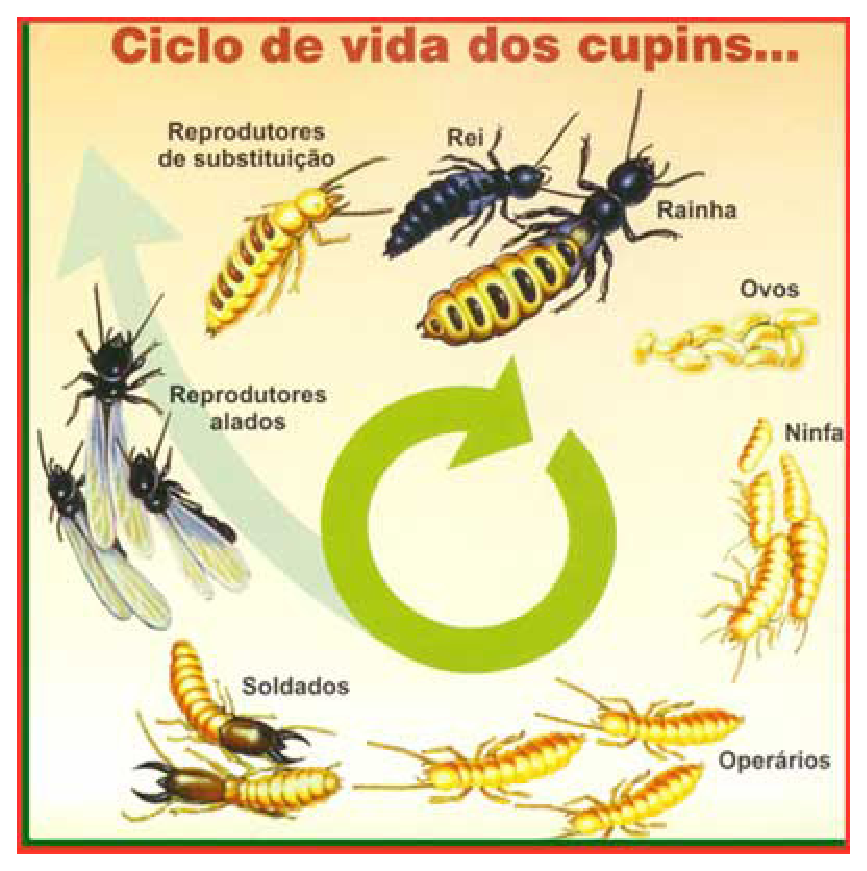
\includegraphics[height=5cm, width=5cm]{ApeA/pragas_ciclo_cupim}
\caption{An illustrative figure included in the appendix.}
\label{fig:example_figure}
\end{figure}

As shown in Figure~\ref{fig:example_figure}, the simulation involves detailed graphical representations to support the findings discussed in the main thesis.



% Anexos--------------------------

\annex %Optional
\chapter{Title for the 1st annex} %optional


Use an annex to include external documents, references, or supplementary materials that, while not integral to the main body of the thesis, provide valuable context or additional support, such as official reports, standards, or other external sources.

\section{Title for This Section}
\label{Ann:Annex}

The following pages include a document in its original format, preserving the content without the need for conversion to images or other forms of manipulation.

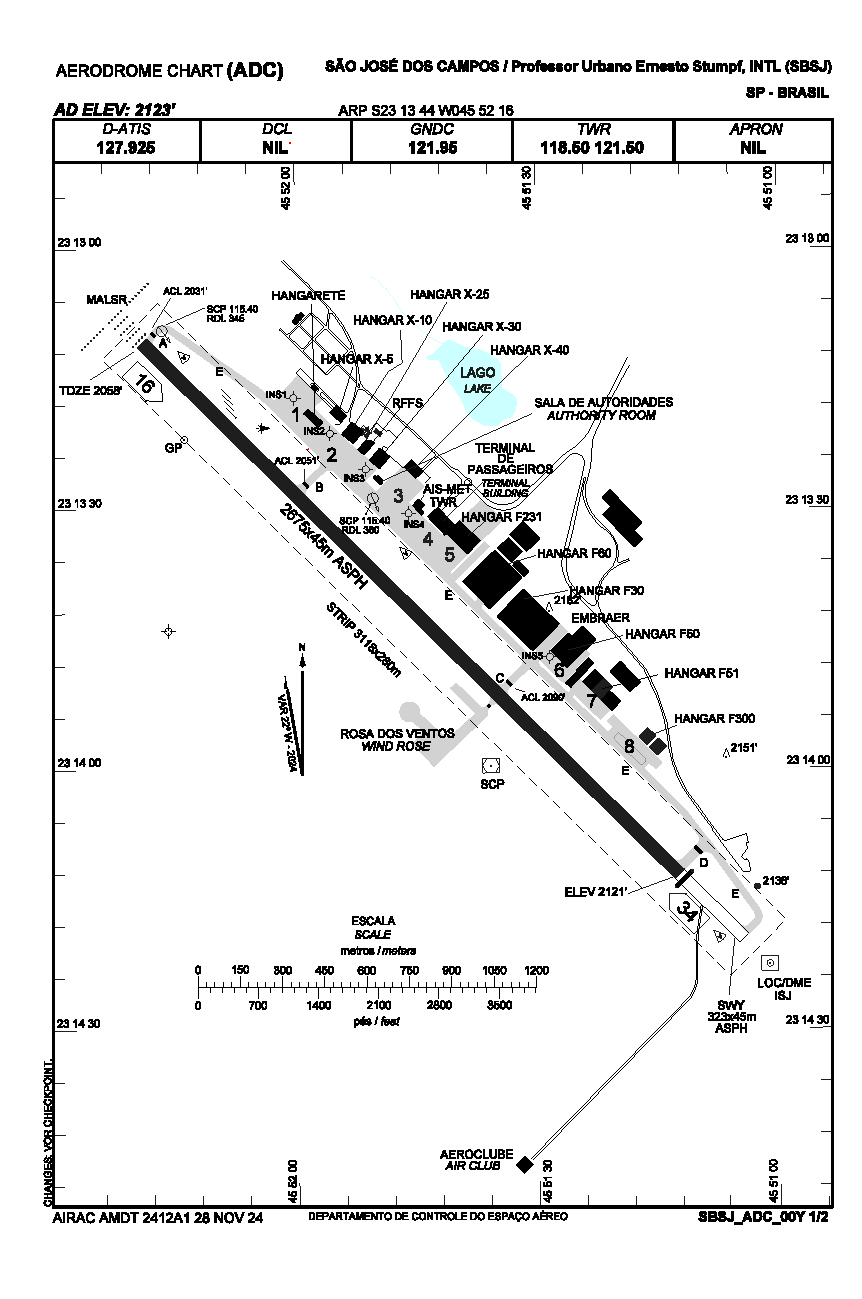
\includepdf[pages=-]{AneA/sbsj_adc-sbsj_adc_20241128.pdf}







%Glossary------------------------------------------

% Glossary Section
% Define a macro for the glossary title based on the language
\newcommand{\itaglosstitle}{%
    \iflanguage{portuguese}{Glossário}{Glossary}%
}

% Glossary Section
\chapter*{\itaglosstitle} % Automatically use "Glossário" or "Glossary"
\addcontentsline{toc}{chapter}{\itaglosstitle} % Add to Table of Contents dynamically



\noindent
\textbf{Document:} A file created using LaTeX for presentation purposes.

\vspace{0.5em}


\noindent
\textbf{Glossary:} A list of terms and their definitions.

\vspace{0.5em}

\noindent
\textbf{LaTeX:} A document preparation system used for high-quality typesetting.

\vspace{0.5em}

\noindent
\textbf{Package:} An add-on feature in LaTeX to enhance its functionality.





%--------------------------------------------------


% Folha de Registro do Documento
% Valores dos campos do formulario
\FRDitadata{25 de março de 2015}
\FRDitadocnro{DCTA/ITA/DM-018/2015} %(o número de registro você solicita a biblioteca)
\FRDitaorgaointerno{Instituto Tecnológico de Aeronáutica -- ITA}
%Exemplo no caso de pós-graduação: Instituto Tecnol{\'o}gico de Aeron{\'a}utica -- ITA
\FRDitapalavrasautor{Cupim; Cimento; Estruturas}
\FRDitapalavrasresult{Cupim; Dilema; Construção}
%Exemplo no caso de graduação (TG):
%\FRDitapalavraapresentacao{Trabalho de Graduação, ITA, São José dos Campos, 2015. \NumPenultimaPagina\ páginas.}
%Exemplo no caso de pós-graduação (msc, dsc):
\FRDitapalavraapresentacao{ITA, São José dos Campos. Curso de Mestrado. Programa de Pós-Graduação em Engenharia Aeronáutica e Mecânica. Área de Sistemas Aeroespaciais e Mecatrônica. Orientador: Prof.~Dr. Adalberto Santos Dupont. Coorientadora: Prof$^\textnormal{a}$.~Dr$^\textnormal{a}$. Doralice Serra. Defesa em 05/03/2015. Publicada em 25/03/2015.}
\FRDitaresumo{É necessário um resumo conciso e objetivo, que não deve ultrapassar 3/4 da página. O resumo deve apresentar brevemente o objetivo da pesquisa, os principais resultados e as conclusões mais relevantes (esperados, parciais ou finais, dependendo do estágio da pesquisa). Como o resumo é frequentemente apresentado separadamente do artigo, ele precisa ser compreensível por si só. Por isso, é recomendável evitar referências; caso sejam indispensáveis, cite o(s) autor(es) e o(s) ano(s). Além disso, abreviações não convencionais ou incomuns devem ser evitadas. Se forem essenciais, devem ser definidas na primeira vez em que aparecerem no próprio resumo.}
%  Primeiro Parametro: Nacional ou Internacional -- N/I
%  Segundo parametro: Ostensivo, Reservado, Confidencial ou Secreto -- O/R/C/S
\FRDitaOpcoes{N}{O}
% Cria o formulario
\itaFRD










\end{document}





%---------------------------------------------------

%%% Modificado em Dez de 2024 por
%%%
%%%   por        Evandro José da Silva   -  evandro [at] ita [dot] br
%%%              Decio Yoshimoto
%%%
%%%
%%% Exemplo de utilização da classe ITA
%%%
%%%   por        Fábio Fagundes Silveira   -  ffs [at] ita [dot] br
%%%              Benedito C. O. Maciel     -  bcmaciel [at] ita [dot] br
%%%              Giovani Volnei Meinertz   -  giovani [at] ita [dot] br
%%%    	         Hudson Alberto Bode       -  bode [at] ita [dot]br
%%%    	         P. I. Braga de Queiroz    -  pi [at] ita [dot] br
%%%    	         Jorge A. B. Gripp         -  gripp [at] ita [dot] br
%%%    	         Juliano Monte-Mor         -  jamontemor [at] yahoo [dot] com [dot] br
%%%    	         Tarcisio A. B. Gripp      -  tarcisio.gripp [at] gmail [dot] com
%%%
%%%   Versão para overleaf:
%%%   por        Alejandro A. Rios Cruz    - aarc.88@gmail.com
%%%              Saulo Gómez               - sagomezs@unal.edu.co
%%%              Ocimar Santos             - ocimar.acad@gmail.com
%%%
%%%   Template disponibilizado em:
%%%              Overleaf: https://pt.overleaf.com/latex/templates/thesis-template-aeronautics-institute-of-technology-ita/yhfrqqydpygk
%%%
%%%   Contribuia você também!
%%%              GitHub:   https://github.com/AlejandroRios/Template_Thesis_ITA
%%%
%%%  IMPORTANTE: O texto contido neste exemplo nao significa absolutamente nada.  :-)
%%%              O intuito aqui eh demonstrar os comandos criados na classe e suas
%%%              respectivas utilizacoes.
%%%
%%%  Tese.tex  2016-08-25
%%%  $HeadURL: https://apgita.org.br/$
%%%
%%% ITALUS
%%% Instituto Tecnológico de Aeronáutica --- ITA, Sao Jose dos Campos, Brasil

%%%
%++++++++++++++++++++++++++++++++++++++++++++++++++++++++++++++++++++++++++++++